%!TEX program = xelatex
\documentclass{article}
\usepackage[UTF8,scheme=plain]{ctex}
\usepackage[a4paper,left=1.25in,right=1.25in,top=1in,bottom=1in]{geometry}

\usepackage{amsmath,amsthm,amsfonts,amssymb}
\usepackage{graphicx}
\usepackage{float}
\usepackage{subcaption}
\usepackage{booktabs,multirow,multicol}
\usepackage{indentfirst}
\usepackage{hyperref}
\usepackage{setspace}
\usepackage{listings}
\usepackage[ruled,noline]{algorithm2e}
\usepackage{bm}
\usepackage{xcolor}

\graphicspath{
    {./figure/}{./figures/}{./image/}{./images/}{./graphic/}{./graphics/}{./picture/}{./pictures/}
}


\title{Lab Report Template}
\author{Author}
\date{\today}

\begin{document}

\maketitle

\section{Introduction}

xxxx.

\section{Method}

xxxx.

\section{Results}

xxxx.

\begin{table}[ht]
    \centering
    \caption{Error and Order Table}\label{tab:demo0}
    \begin{tabular}{c|ccccc}
        \hline
                           & 10       & 20        & 40        & 80         & 160        \\
        \hline
        $L^{\infty}$~error & 0.283284 & 0.0758226 & 0.0192964 & 0.00484029 & 0.00121093 \\
        order              & -        & 1.90      & 1.97      & 2.00       & 2.00       \\
        \hline
    \end{tabular}
\end{table}

\begin{figure}[htbp]
    \centering
    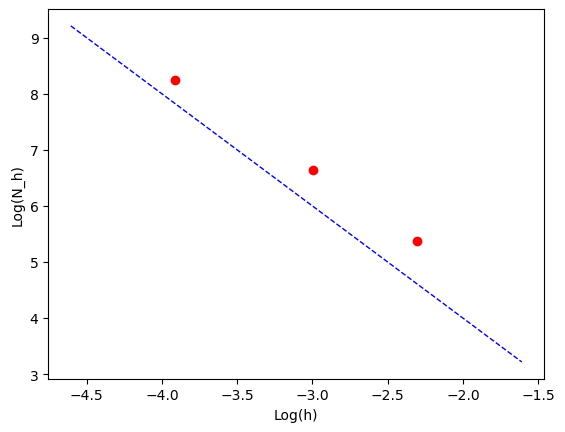
\includegraphics[width=.8\textwidth]{demo1.png}
    \caption{Figure}\label{fig:demo1}
\end{figure}

\begin{figure}[htbp]
    \centering
    \begin{subfigure}[b]{0.47\textwidth}
        \centering
        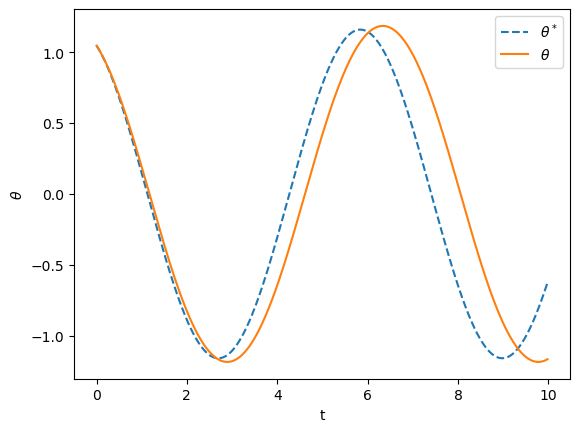
\includegraphics[width=\textwidth]{demo2-1.png}
        \caption{Subfigure 1}
        \label{fig:demo2-a}
    \end{subfigure}
    \begin{subfigure}[b]{0.47\textwidth}
        \centering
        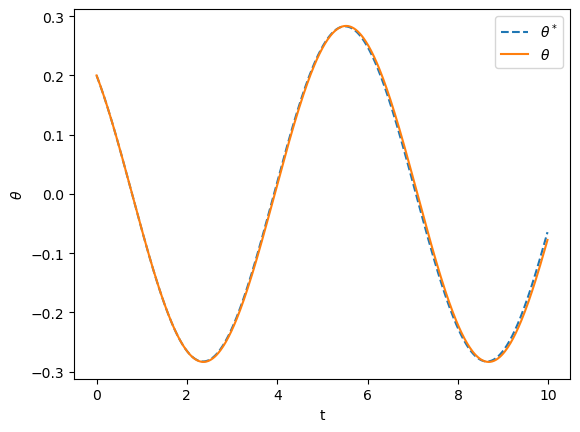
\includegraphics[width=\textwidth]{demo2-2.png}
        \caption{Subfigure 2}
        \label{fig:demo2-b}
    \end{subfigure}
    \caption{Subplots}
    \label{fig:demo2}
\end{figure}

\section{Conclusion}

xxxx.

\end{document}
